\chapter{驱动程序的设计和实现}
	在此我们需要编写一个VxWorks下的USB口转串口的驱动程序,在编写驱动程序之前我们有必要先了解一下VxWorks下驱动的软件结构,USB口转串口的流程以及相关的工作原理。
\section{VxWorks设备驱动概述}
	应用程序必须要通过驱动程序才能够与硬件设备进行通信,而驱动程序的编写与操作系统的关系密不可分。设备驱动程序在操作系统中如何存在、如何与操作系统的其它部分相联系、如何与操作系统的其他部分相联系、如何为用户提供服务都是操作系统的设计人员在设计操作系统时制定的,系统已经为驱动程序制定好了一个框架,无论驱动程序的开发人员以何种方式控制设备,他们所开发的驱动程序都是以预先设计好的方式存在、与操作系统其他部分相联系和为用户提供服务的。将这种由操作系统的设计人员指定的设备驱动程序结构定义为驱动程序的外部结构,而由于驱动开发人员在开发设备驱动时采用的具体策略不同导致的不同的驱动程序结构称为驱动程序的内部结构。驱动程序的外部结构决定了操作系统的I/O体系结构,驱动程序的内部结构决定了不同的设备驱动方式。
	
	驱动程序序简单的说就是设置某个硬件完成其固有功能的程序。驱动程序直接与硬件设备交互,其
大多数的工作就是操作硬件相关寄存器。首先寄存器也是一种 RAM,在系统下电后,寄存器中的内容都会丢失,系统上电复位过程
中,硬件寄存器一般都复位到一个默认值,默认状态下硬件是不能正常工作的,如中断使能
被屏蔽,工作使能位也被屏蔽,还有一些决定硬件工作情况的关键控制寄存器也需要被重新
配置。而这些工作都有赖于设备驱动完成。驱动一般都作为操作系统内核组成的一部分,即
便现在很多系统支持驱动的动态加载,但是驱动代码在执行时,依然是以内核代码模式进行
执行的,换句话说,驱动代码具有系统特权级,除了其自身资源,对应硬件设备资源,其还
对操作系统资源具有完全的访问权。所以一个驱动程序如果存在 BUG,将直接会导致整个
操作系统的崩溃。故调试驱动是一项十分关键的工作,必须对驱动进行仔细检查,并需要经
受长时间运行考验。应用层程序员往往对属于内核编程的外设驱动心存敬畏,认为驱动编程
是一项非常复杂的工作。实际上,底层驱动编程往往比应用层编程具有更大的灵活性,就如
没有调试不出来的硬件,也没有调试不出来的底层驱动,但是应用层 BUG 有时就是无法调
试出来。底层驱动的调试过程是同时对硬件和驱动进行验证的过程。底层驱动很多时候用来
定位硬件设计错误或者硬件芯片本身可能的问题,故底层驱动程序员必须对所要驱动的硬件
设备有一个比较充分的了解,以及对与硬件交互的其他硬件或外界环境也需要有一个比较清
楚的理解。
	
	驱动程序对上需要匹配操作系统提供的一套规范接口,对下必须驱动硬件设备进行工作,其
起着一个关键的中间转换角色,将操作系统的具体请求转换为对硬件的某种操作。驱动程序
在操作系统中扮演着一个非常特殊的角色,其类似一个黑盒子,让所有的硬件对操作系统的
一套内部规范接口进行响应,驱动程序屏蔽了硬件的所有复杂性,应用层对于某个设备的操
作通过操作系统提供的一套标准接口完成,操作系统最终将这些操作请求传递给驱动程序,
驱动硬件完成这些请求。	
	
	
	
	设备驱动时直接控制设备操作的那部分程序,也是设备上层的一个软件接口。设备驱动程序的功能完成软件层对硬件的访问,实际上从软件工程的角度来说就是介于软件和硬件之间实现软件层标准接口的程序。软件层访问硬件必须要通过调用驱动程序。所以驱动程序不能自动执行,只能被系统或者程序调用。
	
	应用程序必须要通过驱动程序才能够与硬件设备进行通信,而驱动程序的编写与操作系统的关系密不可分。设备驱动程序在操作系统中如何存在、如何与操作系统的其它部分相联系、如何与操作系统的其他部分相联系、如何为用户提供服务都是操作系统的设计人员在设计操作系统时制定的,系统已经为驱动程序制定好了一个框架,无论驱动程序的开发人员以何种方式控制设备,他们所开发的驱动程序都是以预先设计好的方式存在、与操作系统其他部分相联系和为用户提供服务的。将这种由操作系统的设计人员指定的设备驱动程序结构定义为驱动程序的外部结构,而由于驱动开发人员在开发设备驱动时采用的具体策略不同导致的不同的驱动程序结构称为驱动程序的内部结构。驱动程序的外部结构决定了操作系统的I/O体系结构,驱动程序的内部结构决定了不同的设备驱动方式。

	在VxWorks系统中,在控制器权转到设备驱动程序之前,用户的请求进行尽可能少的处理。VxWorks I/O系统的角色更像是一个转接开关,负责将用户请求转接到合适的驱动例程上。每一个驱动都能够处理原始的用户请求,到最合适它的设备上。另外,驱动程序开发者也可以利用高级别的库例程来实现基于字符设备或者块设备的标准协议。因此,VxWorks的I/O系统具有两方面的优点:一方面使用尽可能少的使用驱动相关代码就可以为绝大多数设备写成标准的驱动程序,另一方面驱动程序开发者可以在合适的地方使用非标准的程序自主的处理用户请求。





\subsection{设备驱动的功能以及分类}\label{sec:设备分类}
	驱动程序是位于用户和硬件之间一个软件层,驱动程序员有完全的决定权决定一个硬件设备以何种形式呈现给用户,不同的驱动程序可以使得同一个硬件设备以不同的方式对用户可见。我们可以将一个实际块设备以字符设备对用户可见,将一个实际Flash设备以硬盘设备对用户可见,以何种形式表现一个实际设备完全由底层驱动控制。驱动程序员可以提供一系列方式让用户对设备进行控制,甚至可以让用户直接操作硬件设备的每一个寄存器,由用户在寄存器层次对硬件设备进行操作;或者只提供一个读或写操作,屏蔽其他所有操作等等。
	
	故从宏观角度而言,驱动程序实现的功能即提供一种底层服务机制供用户进行选择。从微观角度而言,驱动程序需要对下配置硬件寄存器,完成对设备数据的读写,对设备本身的控制,对上使得设备能够响应用户的服务请求,这些服务请求如下:打开设备;读写设备;控制设备;关闭设备。

	根据设备的工作方式和数据的存储或者来源不同,可以将设备分为三大类:
\begin{itemize}
\item \hei{字符设备类型}

	字符设备即以字节流的方式被访问,就如同一个文件,但不同于文件之处是字符设备一般不可以移动文件偏移指针,而只能顺序的访问数据。终端设备以及串口设备都属于字符设备类型。字符设备驱动至少需要实现 open,close,read 和 write 四个系统调用底层实现函数。

\item \hei{块设备类型}

	块设备一般通过文件系统访问。而块设备的最多使用方式也是文件方式。块设备一般不能对单个字节进行访问,而是一个块的方式(如硬盘以一个扇区(512B)为单元进行访问)进行。块设备允许同一数据的反复读取和写入。最典型的块设备就是硬盘,Flash 设备也是一种块设备。
	
\item \hei{网络设备类型}

	用于与网络上其他主机进行通信。其数据读取方式有些类似于字符设备,不可以对同一数据进行反复读写,只能顺序读写数据。且该类型设备区别于字符设备和块设备的一个很大的不同是,其不提供文件节点,任务要访问一个网络设备必须使用另一套网络套接字接口函数进行,与文件系统则完全不相关。网络设备底层数据传输上以块的方式进行,但是又不同于块设备中数据块的概念,网络设备中块的大小可以改变,但是有一个区间范围。
\end{itemize}

	以上只是设备类型的划分方式之一,事实上,按以上的划分标准,某些设备接口在某些情况下可以表现为任意以上三种形式之一,如 USB 接口,可以是一个字符设备,如 USB 串口;也可以是一个块设备,如 USB 内存卡;也可以是一个网络设备,如 USB 网络接口。

\subsection{VxWorks设备驱动层次结构}
	VxWorks 的I/O框架由ioLib.c 文件提供,但ioLib.c文件提供的函数仅仅是一个最上层的接口,并不能完成具体的用户请求,而是将请求进一步向其他内核模块进行传递,位于ioLib.c模块之下的模块就是iosLib.c。我们将ioLib.c 文件称为上层接口子系统,将iosLib.c文件称为I/O 子系统,注意二者的区别。上层接口子系统直接对用户层可见,而I/O 子系统则一般不可见(当然用户也可以直接调用iosLib.c 中定义的函数,但一般需要做更多的封装,且违背了内核提供的服务层次),其作为上层接口子系统与下层驱动系统的中间层而存在。VxWorks的内核驱动层次结构如\autoref{fig:VxWorks内核驱动层次结构}所示。
\begin{figure}[!h]
\centering
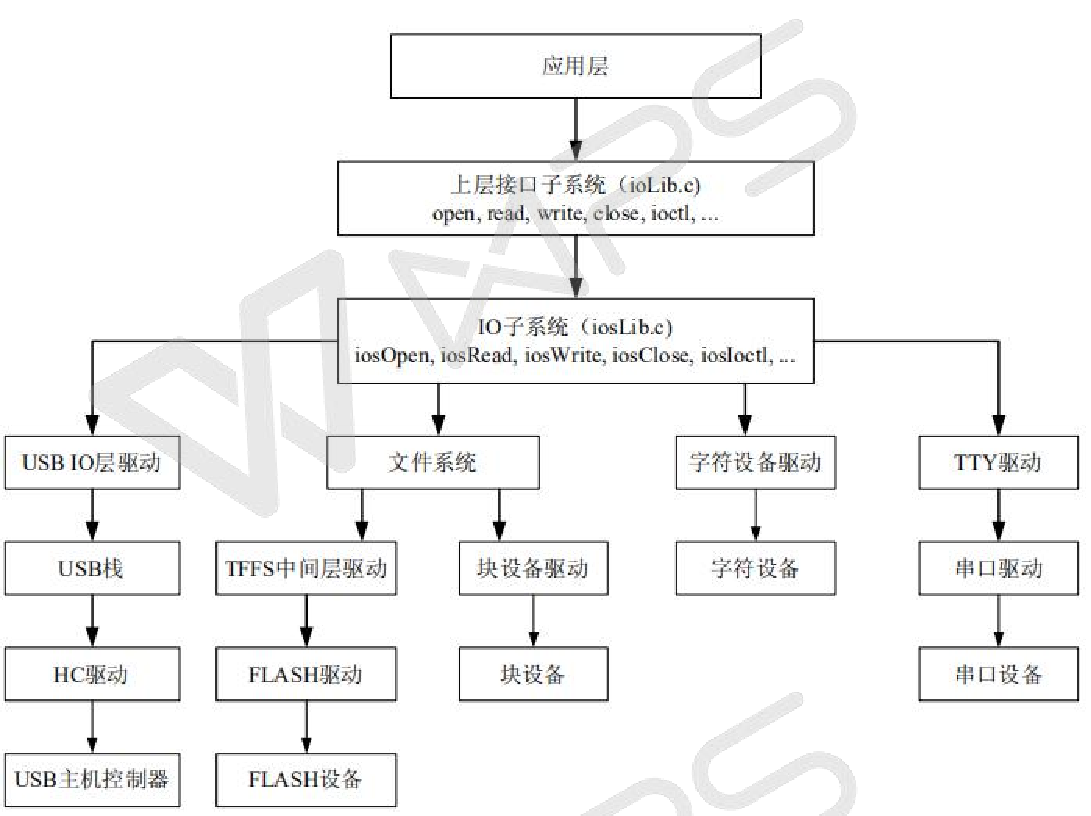
\includegraphics[width=1.0\textwidth]{./graphics/vxworks-kernel-diagram.pdf}
\caption{VxWorks驱动内核层次结构}\label{fig:VxWorks内核驱动层次结构}
\end{figure}

	

	I/O 子系统在整个驱动层次中起着十分重要的作用,其对下管理着各种类型的设备驱动。换句话说,各种类型(包括网络设备)的设备都必须向I/O 子系统进行注册方可被内核访问。所以在I/O 子系统这一层次,内核维护着三个十分关键的数组用以对设备所属驱动、设备本身以及当前系统文件句柄进行管理。

	需要指出的是,VxWorks文件系统在内核驱动层次中实际上是作为块设备驱动层次中的一个中间层而存在的,其向I/O 子系统进行注册,而将底层块设备驱动置于自身的管理之下以提高数据访问的效率。在这些文件系统中,dosFs 和rawFs 是最常用的两种文件系统类型,在VxWorks早期版本就包含对这两种文件系统的支持。
	
\section{内核驱动的相关结构}
\subsection{系统设备表}
	
	在VxWorks中对于每一个设备都会使用DEV\_ HDR的结构来表示这个设备,DEV\_ HDR的定义如下:
\lstset{language=C}
\begin{lstlisting}
/*h/iosLib.h*/
typedef struct /* DEV_HDR - device header for all device structures */ 
{ 
  DL_NODE node; /* device linked list node */ 
  short drvNum; /* driver number for this device */ 
  char * name;/* device name */ 
}DEV_HDR;  
\end{lstlisting}

	在该结构中给出了链接指针node(用以将该结构串入队列中),驱动索引号drvNum,设备节点名name。内核提供这个结构较为简单,只存储了一些设备关键部分。底层驱动对其驱动的设备都有一个自定义数据结构表示,其中包含了被驱动设备寄存器基地址,中断号,可能的数据缓冲区,保存内核回调函数的指针,以及一些标志位。最为关键的一点是 DEV\_ HDR 内核结构必须是这个自定义数据结构的第一个成员变量,因为这个用户自定义结构最后需要添加到系统设备队列中,故必须能够在用户自定义结构与 DEV\_ HDR 结构之间进行转换,而将 DEV\_ HDR 结构设置为用户自定义结构的第一个成员变量就可以达到这个目的。
	
	为了能够让用户对设备进行操作,驱动程序必须将设备注册到 IO 子系统中,这个过程也被称为创建设备节点。IO子系统提供了一个简单的被驱动程序调用的设备注册函数iosDevAdd(),该函数原型如下:
\lstset{language=C}
\begin{lstlisting}
STATUS iosDevAdd 
( 
  DEV_HDR *pDevHdr, /* pointer to device's structure */ 
  char *name, /* name of device */ 
  int drvnum /* no. of servicing driver,returned by iosDrvInstall()*/
 ); 
\end{lstlisting}

iosDevAdd 函数将一个设备添加到由 IO 子系统维护的系统设备列表中,该列表是一个队列,队列中成员通过指针链接在一起,这是由 DEV\_ HDR 结构中 node 成员变量完成的。系统设备列表由 iosDvList 内核变量指向,系统设备表在系统中的连接方式如下\autoref{fig:VxWorks系统设备示意图}所示:

\begin{figure}[!h]
\centering
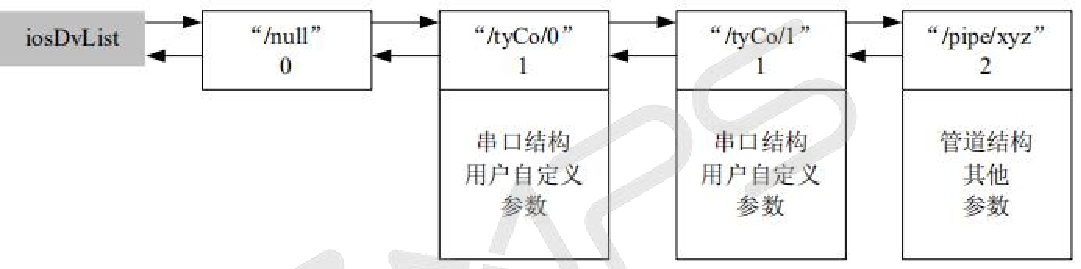
\includegraphics[width=1.0\textwidth]{./graphics/vxworks-device-link.pdf}
\caption{VxWorks系统设备示意图}\label{fig:VxWorks系统设备示意图}
\end{figure}

用户可以在命令行下使用iosDevShow或者是devs来显示系统设备的所有设备,在本次使用的环境中,存在的设备如\autoref{fig:iosDevShow}所示。
\begin{figure}[!h]
\centering
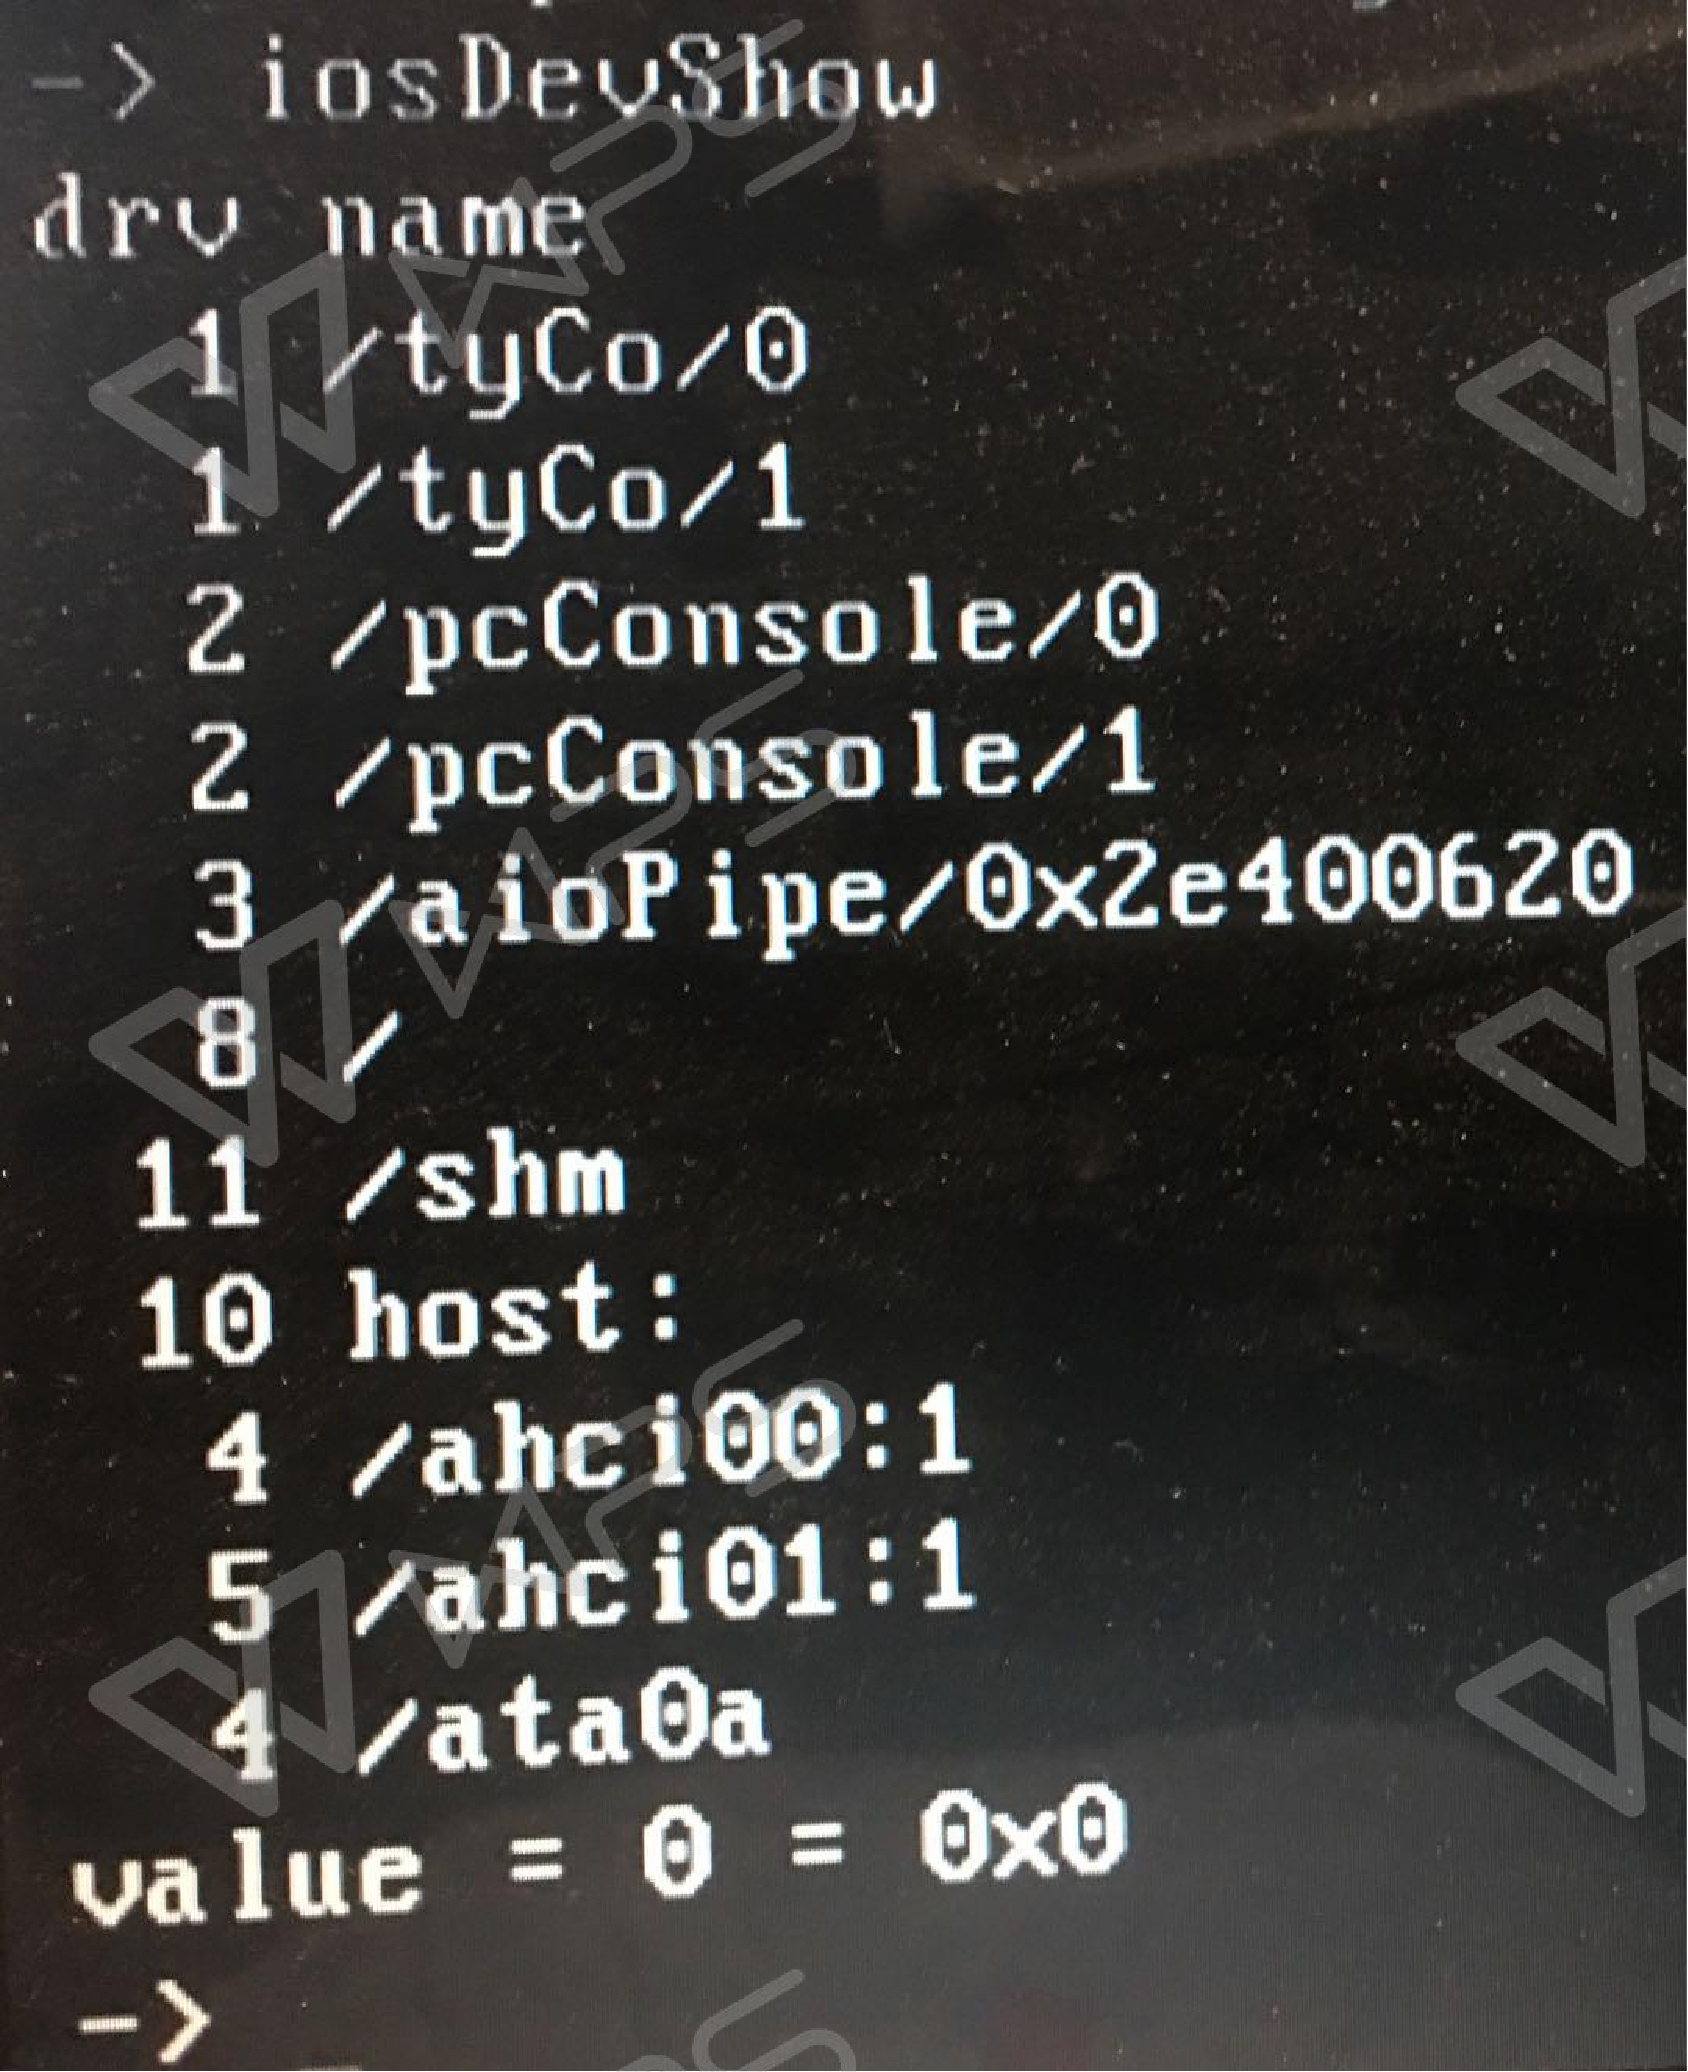
\includegraphics[width=.5\textwidth]{./graphics/iosDevShow.pdf}
\caption{当前系统上的所有设备}\label{fig:iosDevShow}
\end{figure}

\subsection{系统驱动表}
	IO子系统维护的系统驱动表包含有当前注册到IO子系统下的所有驱动。这些驱动可以是直接驱动硬件工作的驱动层,如一般的字符驱动,也可以是驱动中间层,如文件系统中间层,TTY 中间层,USB IO 中间层等。对于中间层驱动,下层硬件驱动将由这些中间层自身负责管理,而不再通过 IO 子系统。如串口底层驱动将通过 TTY 中间层进行管理,而不再通过IO 子系统。

	系统驱动表底层的实现是一个数组,数组元素数目在 Vxworks 内核初始化过程中初始化 IO 子系统时指定,iosInit()函数用以初始化 IO 子系统,我们在编写驱动程序的时候不需要再调用此函数,因为内核已经帮我们初始化好了 IO 子系统。iosInit 函数调用原型如下:
\lstset{language=C}
\begin{lstlisting}
STATUS iosInit 
( 
  int max_drivers, /* maximum number of drivers allowed */ 
  int max_files, /* max number of files allowed open at once */ 
  char *nullDevName/* name of the null device (bit bucket) */ 
); 
\end{lstlisting}

在系统的驱动表中每一个表项都是一个 DRV\_ ENTRY 类型的结构,该结构定义在 h/private/iosLibP.h文件当中,其定义如下:
\lstset{language=C}
\begin{lstlisting}
typedef struct /* DRV_ENTRY - entries in driver jump table */ 
{ 
  FUNCPTR de_create; 
  FUNCPTR de_delete; 
  FUNCPTR de_open; 
  FUNCPTR de_close; 
  FUNCPTR de_read; 
  FUNCPTR de_write; 
  FUNCPTR de_ioctl; 
  BOOL de_inuse; 
} DRV_ENTRY; 
\end{lstlisting}
DEV\_ ENTRY结构体实际上就是一个函数指针结构,结构中每个成员都指向一个完成特定功能的函数,这些函数与用户层提供标准函数接口一一对应。成员 de\_ inuse 用以表示一个表项是否空闲。这个结构体中的函数指针实际指向的内容由驱动调用iosDrvInstall()来提供。 iosDrvInstall()是IO子系统提供的驱动程序注册函数,其原型如下:
\lstset{language=C}
\begin{lstlisting}
int iosDrvInstall 
( 
  FUNCPTR pCreate, /* pointer to driver create function */ 
  FUNCPTR pDelete, /* pointer to driver delete function */ 
  FUNCPTR pOpen, /* pointer to driver open function */ 
  FUNCPTR pClose, /* pointer to driver close function */ 
  FUNCPTR pRead, /* pointer to driver read function */ 
  FUNCPTR pWrite, /* pointer to driver write function */ 
  FUNCPTR pIoctl /* pointer to driver ioctl function */ 
); 
\end{lstlisting}
一个设备驱动在初始化过程中一方面完成硬件设备寄存器的配置,另一方面就是向 IO 子系统注册驱动和设备,从而使得设备对用户可见。可以看到 iosDrvInstall 函数参数为一系列函数地址,这些函数对应了为用户层提供的标准接口函数。一个驱动无需提供以上所有函数的实现,对于无需实现的函数,直接传递 NULL 指针即可。iosDrvInstall 函数基本实现即遍历drvTable 数组,查询一个空闲表项,用传入的函数地址对表项中各成员变量进行初始化,并将 de\_ inuse 设置为 TRUE,最后返回该表项在数组中的索引作为驱动号。设备初始化函数将使用该驱动号调用 iosDevAdd 将设备添加到 IO 子系统中。此后用户就可以使用 iosDevAdd函数调用时设置的设备节点名对设备进行打开操作,打开后进行读写或控制等其他操作,完成用户要求的特定功能。

	用户可在命令行下输入 iosDrvShow,显示系统驱动表中当前存储的所有驱动。如\autoref{fig:iosDrvShow}所示为当前系统中的所有驱动。
\begin{figure}[!h]
\centering
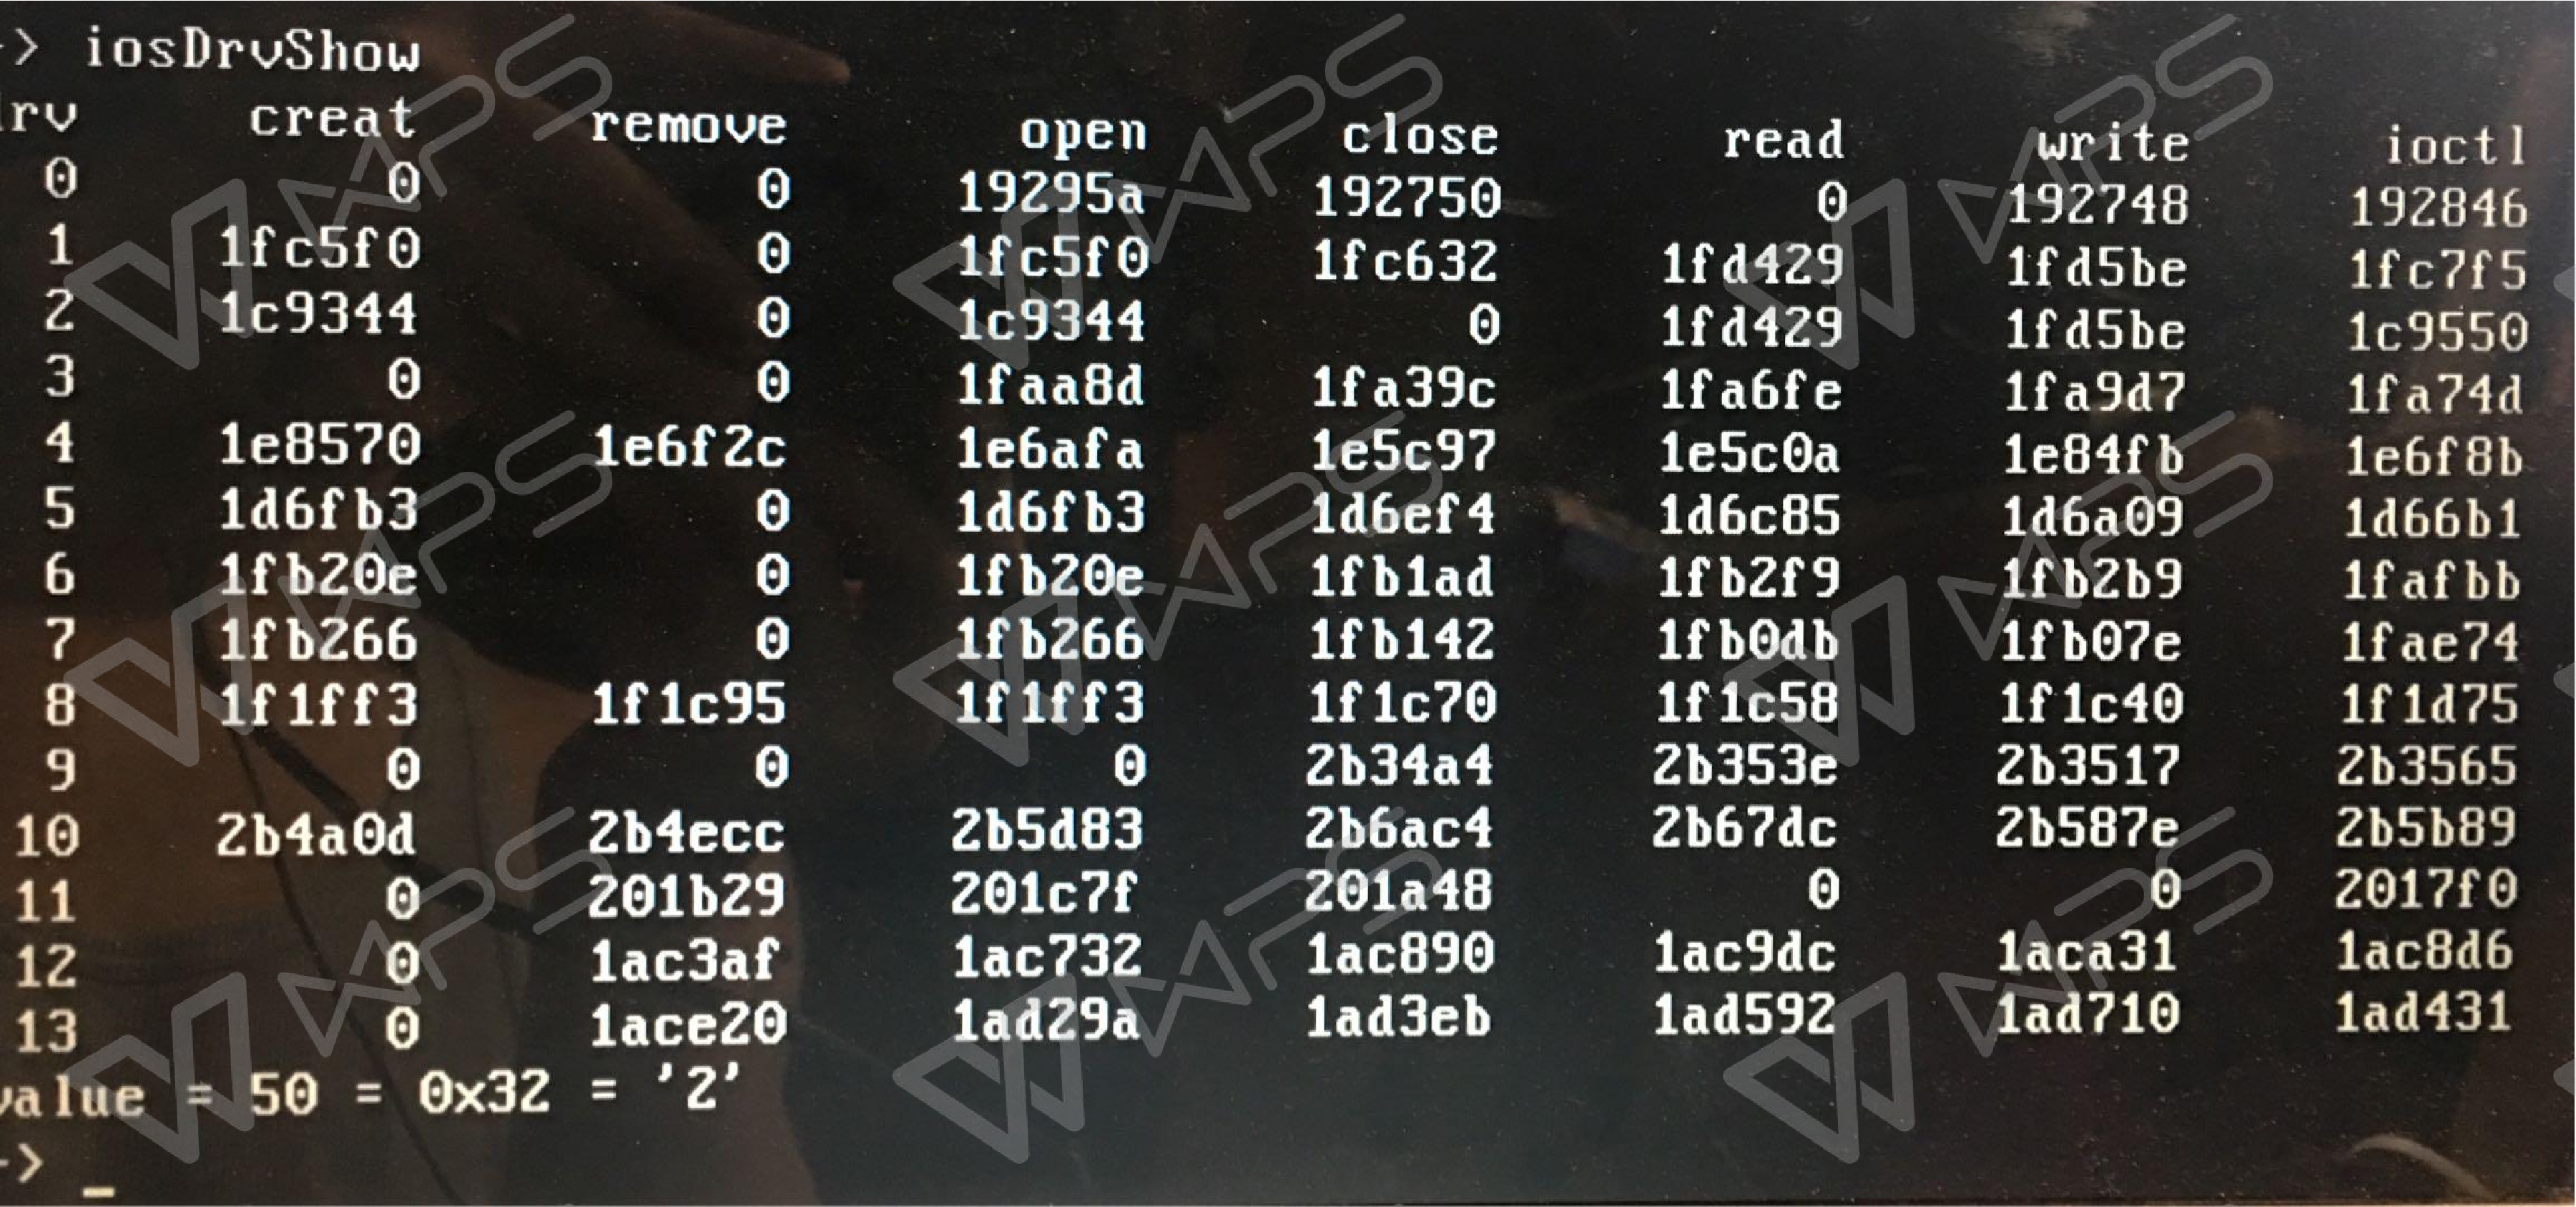
\includegraphics[width=.9\textwidth]{./graphics/iosDrvShow.pdf}
\caption{当前系统上的驱动表}\label{fig:iosDrvShow}
\end{figure}

\subsection{系统文件描述符表}
	系统描述符表存储着当前系统范围内打开的所有文件的描述符。文件描述符表底层实现上也是一个数组,正如设备驱动表表项索引用作驱动号,文件描述符表表项索引被用作文件描述符 ID,即 open 函数返回值。对于文件描述符有一点需要注意:标准输入,标准输出,标准错误输出虽然使用 0,1,2 三个文件描述符,但是可能在系统文件描述附表中只占用一个表项,即都使用同一个表项。Vxworks 内核将 0,1,2 三个标准文件描述符与系统文件描述符表中内容分开进行管理。实际上系统文件描述符中的内容更多的是针对硬件设备,即使用一次 open 函数调用就占用一个表项。0,1,2 三个标准文件描述符虽然占用 ID 空间(即其他描述符此时只能从 3 开始分配),但是其只使用了一次 open 函数调用,此后使用 ioGlobalStdSet 函数对 open 返回值进行了复制。
	
	系统文件描述符表中每个表项都是一个 FD\_ ENTRY 类型的结构,该结构定义在h/private/iosLibP.h 中,如下所示。
\lstset{language=C}
\begin{lstlisting}
typedef struct /* FD_ENTRY - entries in file table */ 
{ 
  DEV_HDR * pDevHdr;/* device header for this file */ 
  int value; /* driver's id for this file */ 
  char * name; /* actual file name */ 
  int taskId; /* task to receive SIGIO when enabled */ 
  BOOL inuse; /* active entry */ 
  BOOL obsolete; /* underlying driver has been deleted */ 
  void * auxValue;/* driver specific ptr, e.g. socket type */ 
  void * reserved; /* reserved for driver use */ 
} FD_ENTRY; 
\end{lstlisting}

用户程序每调用一次 open 函数,系统文件描述符表中就增加一个有效表项,直到数组满,此时 open函数调用将以失败返回。表项在表中的索引偏移 3 后作为文件描述符返回给用户,作为接下来其他所有操作的文件句柄。用户可以通过iosFdShow来显示系统文件描述符表中当前所有的有效表项,如\autoref{fig:iosFdShow}所示是当前系统下的文件系统描述符表。
\begin{figure}[!h]
\centering
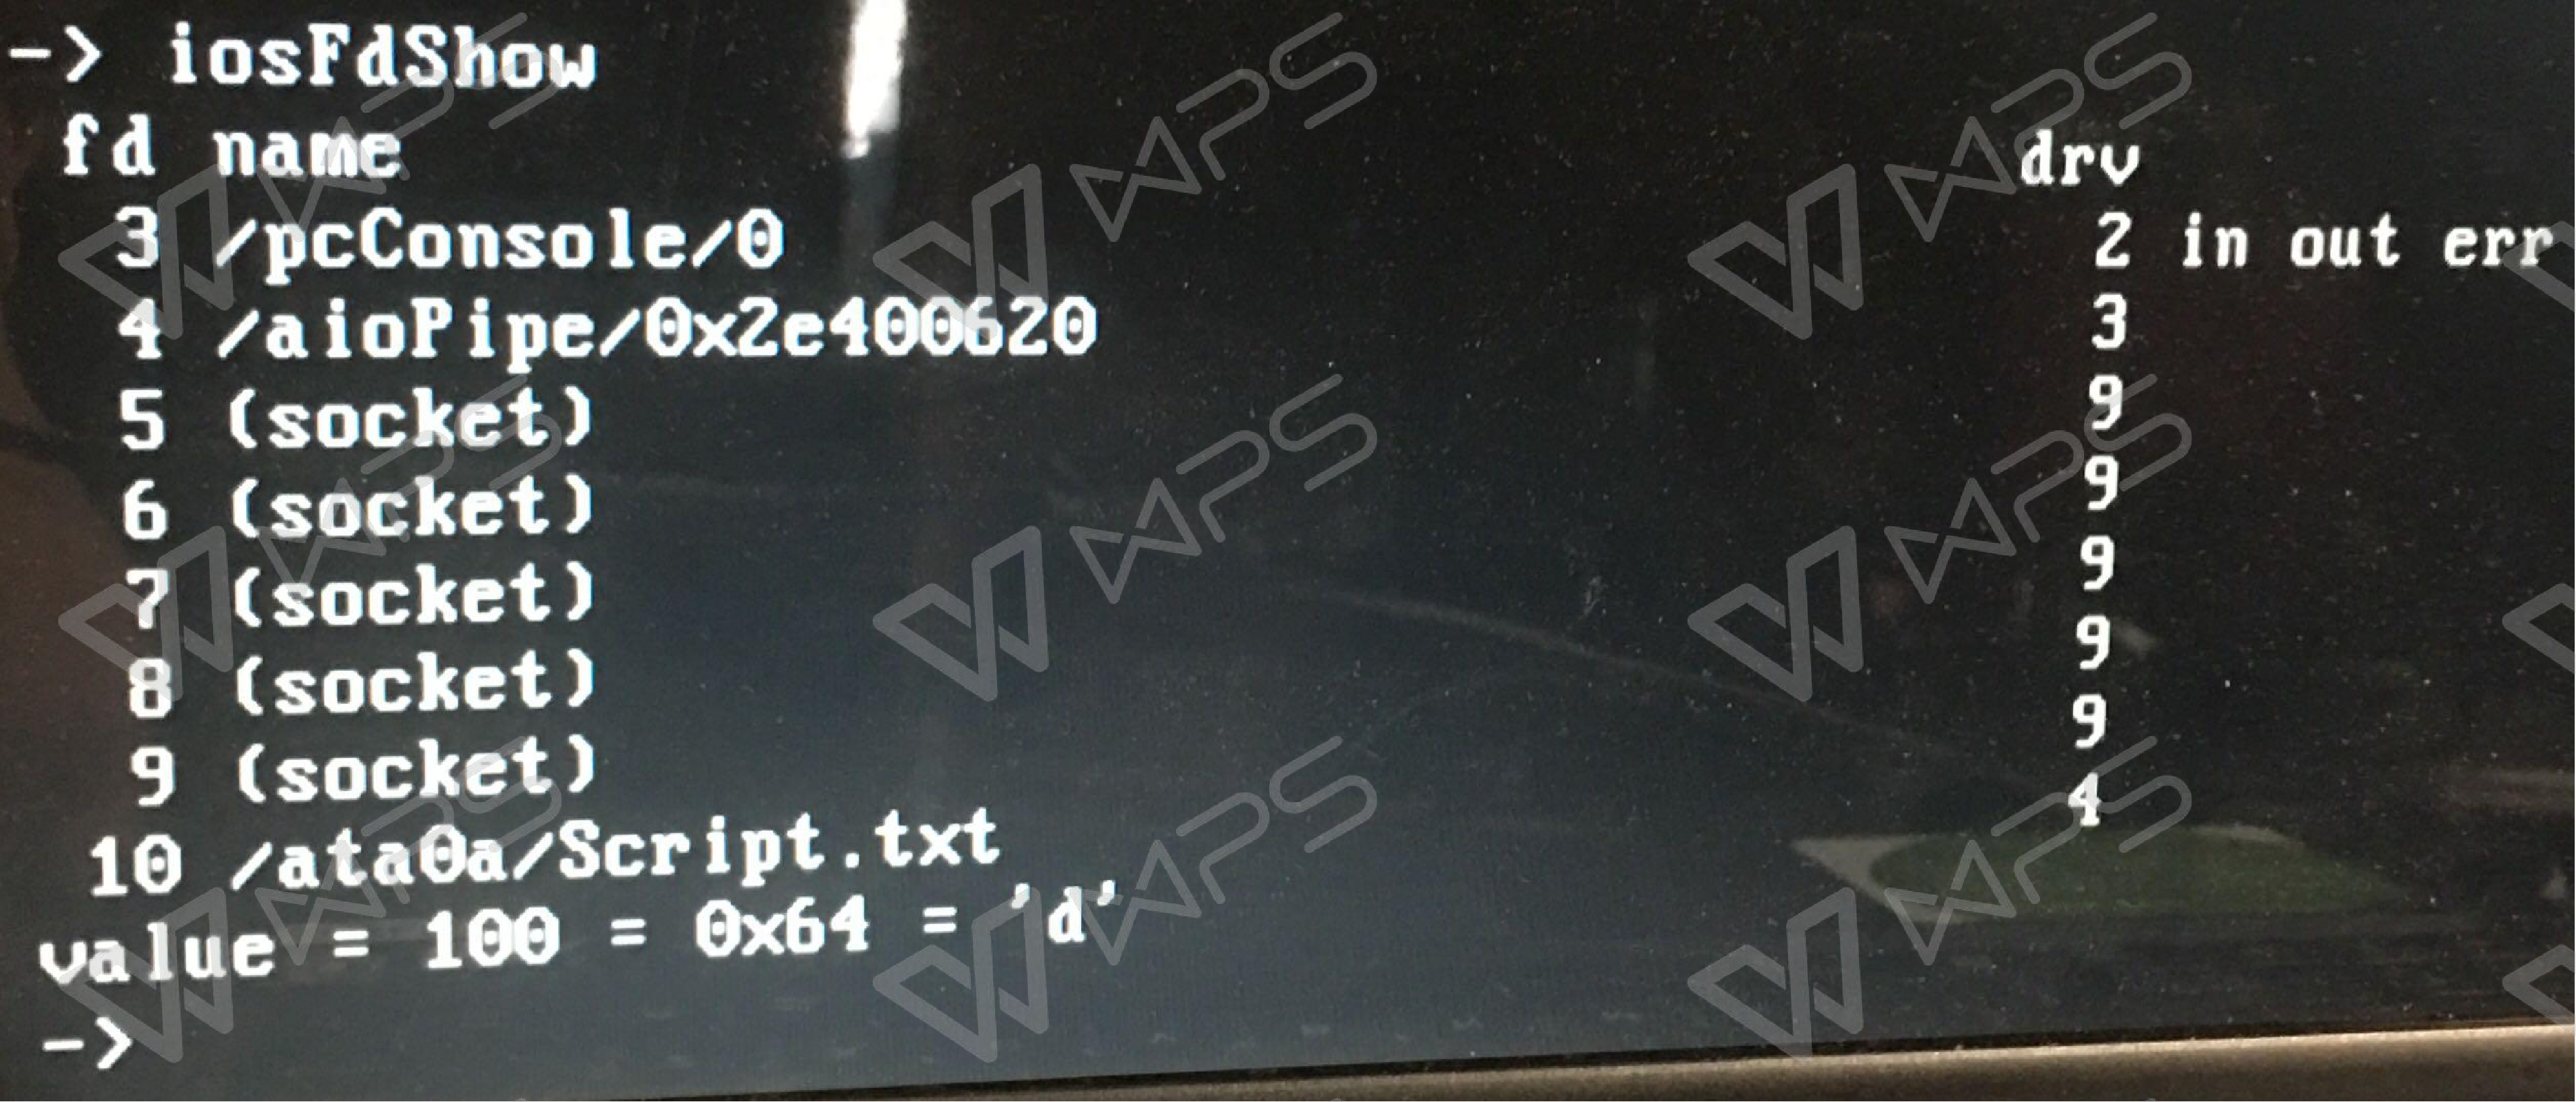
\includegraphics[width=.9\textwidth]{./graphics/iosFdShow.pdf}
\caption{当前系统上的文件描述符表}\label{fig:iosFdShow}
\end{figure}

\section{USB转串口设备驱动程序的实现}
	VxWorks调试通道当中运行的最主要的软件平台是嵌入式实时操作系统VxWorks,作为系统的最底层的软件,要想进行数据的传输,驱动程序是必不可少的。本系统中的硬件设备是基于USB总线的,USB口转串口设备的驱动程序在Windows和Linux下都有现成可用的,但是在VxWorks下需要自己来实现这部分。
	
	
	
	在应用程序可以与一个设备通信之前,主机需要知道设备支持哪一些传输类型和终端,主机也必须要分配一个地址给设备。主机通过一个被称为列举的信息交换来完成这些工作。以下叙述USB列举的基本过程:
\begin{enumerate}
\item \hei{USB设备与主机系统的交互}

	MCU对USB芯片进行初始化:设置内部时钟,选择内部连接方式以及是否开通DMA传输等;设定设备的工作模式,并设备本设备的初始地址为0(USB规范指明当设备接入PC的时候都由初始为0的地址对主机进行响应,之后再由主机分配一个地址给USB设备,设备接收到分配地址命令后,再更改自己的地址,并一直通过这个地址完成后续的通信)。
	完成初始化工作之后,MCU将使能USB接口,主机系统将因此检测到一个新的USB接入而很快与设备进行握手,获取设备的基本信息,并完成一些列的对设备的配置,其过程为:
	\begin{enumerate}
	\item USB上电使能后,主机会向USB设备发送GET DEVICE DESCRIPTOR的命令,之后主机会收到设备发出的设备描述符,随即为设备分配一个空闲地址,并向设备发送SET ADDRESS的命令,这时设备通过地址0发送一个长度为0的数据包予以应答,然后根据主机的要求更改自身的地址,而且这以后的数据交换都将会通过这个新的地址来进行。
	\item 完成地址设备之后,主机将会发送GET CONFIGURATION DESCRIPTOR,USB规定当主机发出该命令符的时候,设备必须要同时返回配置所包含的所有接口和接口所包含的所有端点的描述符。
	\item 主机获取到USB设备的描述符、配置描述符并进行了地址设置之后,设备与主机的握手初步完成,之后会将该设备加入到设备列表当中。
	\end{enumerate}
	
	\item \hei{USB设备与驱动程序的交互}
	
USB设备的驱动与传统意义上的硬件驱动不完全相同,他并不与硬件直接通信,而是以创建和发送URB请求块的形式把命令传递给操作系统所提供的USB总线驱动程序,由总线驱动程序来完成与硬件的直接交互。和主机类似,驱动会首先创建和发送请求得到该设备的DEVICE DESCRIPTOR的URB,并将获取到的信息存储在专用的数据结构当中,接着驱动为了得到完整的设备配置,必须要通过总线驱动发送两次GET CONGFIGURATION DESCRIPTOR命令得到设备。获取设备的配置信息之后,驱动在启动设备之前还要发送SET CONFIGURATION、SET INTERFACE命令。通过以上的几个步骤便可以完成驱动与USB设备过程。	
\end{enumerate}

	当设备接入到PC的USB接口的时候,在固件和操作系统的支持下会对设备进行枚举操作,
	
	由于我们的USB驱动程序不能够支持处理中断,所以只能够用查询的方式来连续接收数据。可以使用两种方式实现设备的查询,一是使用计时器,另外就是使用系统线程。在我们的USB口转串口驱动程序中,我们使用两个线程实现数据的接收操作。在第一次设置PID过滤参数之后,开启一个系统线程,它会不停的从IN端口读取数据,然后写入到驱动程序中开辟的缓冲区当中;

\subsection{VxWorks上的USB协议栈}
	VxWorks的USB主机驱动程序堆栈满足USB协议规定的要求,提供了一整套服务来操作USB以及一些预置USB类驱动程序,以处理特定类型的USB设备。在Wind River的VxWorks中USB驱动程序堆栈的开发符合的是通用串行总线规范2.0版,USB系统是一种主从结构,系统的所有动作都是由USB主机发起,并协调不同的设备动作,设备端软件在系统中只需要对主机的命令做出响应即可,USB的主机端由于在系统中的地位比较特殊,因而其软件结构比较复杂,USB协议在主机端是分层实现的,其通信的逻辑结构和PC端的软硬件结构如\autoref{fig:usb通信结构}所示。USB协议由上至下可以分为三层:客户端驱动程序(Client Driver)、USB驱动(USBD)、主机控制器驱动(HCD),每一层完成不同的功能。

\begin{figure}[h]
\centering
  \begin{subfigure}[b]{0.4\textwidth}
  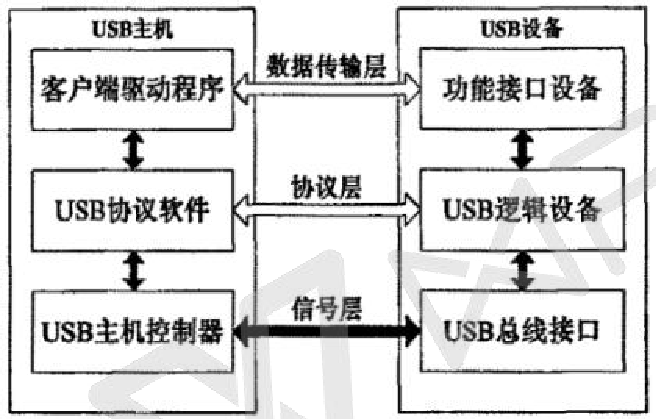
\includegraphics[width=1.0\textwidth]{./graphics/USB-device-structure-diagram.pdf}
  \caption{USB通信的逻辑结构}\label{fig:usb通信逻辑结构}
  \end{subfigure}
  ~
  \begin{subfigure}[b]{0.5\textwidth}
  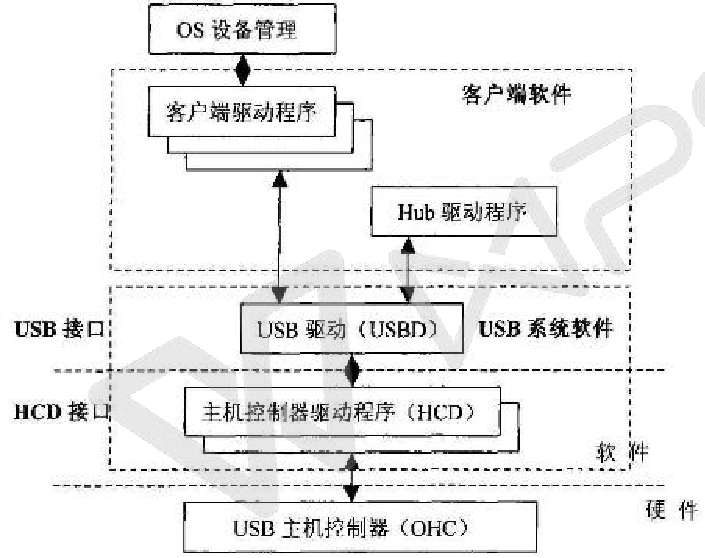
\includegraphics[width=1.0\textwidth]{./graphics/USB-PC-structure.pdf}
  \caption{USB主机端软硬件结构}\label{fig:usb-PC}
  \end{subfigure}
\caption{USB通信结构}\label{fig:USB通信结构}
\end{figure}

	客户端驱动程序完成对不同的设备类的设备的功能驱动。本次设计中所要完成的USB口转串口的驱动要完成的就是客户端驱动。为了和设备进行正常的通信,他通过USB的I/O请求包(I/O request,IRP)向USBD层发出数据接收或者发送的请求。此外,USB的传输机制对于客户端的驱动程序而言是完全透明的,客户端驱动程序所看到的仅仅是具体的设备类,不管设备采用的何种的数据传输方式。另外IRP是USB协议定义的抽象概念,其结构需要根据协议的具体来实现。
	
	USBD主要负责处理客户端驱动程序提供的I/O请求,他通过IRP知道此设备的属性和本次数据通信的具体要求,将此IRP转换成USB能够识别的一系列的事物处理,交给HCD层或直接交给主机控制器处理。USBD还负责新设备的检测和配置、被拔掉的设备的资源释放和对客户端驱动程序的维护等操作。
	
	HCD层的主要功能是与主机控制器合作完成USB的各种事物处理。它根据一定的规则调度所有奖杯广播发送到USB上的事物处理。调度方法是首先将数据传输类型组成不同的链表,每一种链表包括来自不同的设备驱动程序的同一种类型的数据,然后定义不同的数据类型在传输中所占的带宽比例,交给主机控制器处理,控制器根据规则从立案表上摘下数据块,根据大小为它创建一个或者多个事物处理,完成与设备的数据传输,当事物处理完成时HCD将结果交给USBD层。此外它还完成对主机控制器和根集线器的配置和驱动等操作。


\subsection{特定需求的单设备支持}

	由于对于仅支持单设备驱动程序是基于特定的需求而具体定制的,所以该设备的驱动程序的实现流程与标准的设备的驱动的初始化流程存在差异。具体的需求为:
\hei{驱动中支持的设备名是固定的,驱动程序中要有缓存一定数据的能力,即使设备没有正确的连接也要能够往这个驱动中写入数据,并且一旦设备连接之后就能够将驱动中缓存的数据发送出去。}

	由于需要在设备未连接时就能够往设备中写入数据,且设备名为固定的,那么就必须调整驱动的初始化流程,使得其能够支持这一特性,通常驱动都是在设备加载之后再将其加入到系统设备表和系统驱动表当中,那么此时我们就需要先将一个固定的设备名加入到系统设备表当中。对于该特定需求的单设备驱动的流程图如\autoref{fig:single-usb-rs232drv-structure}所示。
\begin{figure}[!h]
\centering
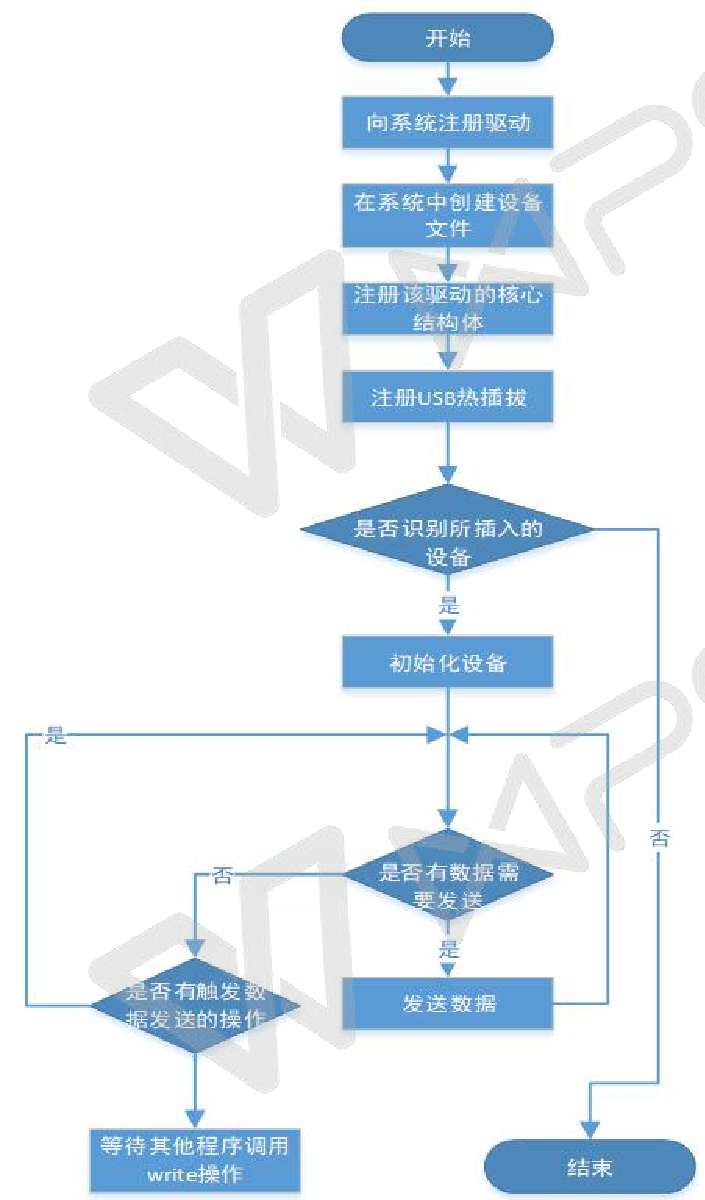
\includegraphics[width=.9\textwidth]{./graphics/single-usb-rs232drv-structure.pdf}
\caption{特定需求的驱动流程图}\label{fig:single-usb-rs232drv-structure}
\end{figure}
	
	
	

驱动程序各模块的实现:
\begin{enumerate}
\item  cp210xDevInit模块

	

\end{enumerate}


\subsubsection{USB设备硬件的初始化}


\subsection{通用的多设备支持}